\documentclass[a4paper,11pt,twoside]{article}
\usepackage[T1]{fontenc}
\usepackage{subcaption}
\usepackage[utf8]{inputenc}
\usepackage{ngerman, eucal, mathrsfs, amsfonts, bbm, amsmath, amssymb, stmaryrd,graphicx, array, geometry, color, wrapfig}
\geometry{left=25mm, right=15mm, bottom=25mm}
\setlength{\parindent}{0em} 
\setlength{\headheight}{0em} 
\title{Machine Learning\\ Blatt 2}
\author{Markus Vieth, David Klopp, Christian Stricker}
\date{\today}
\usepackage{listings, textcomp}
\usepackage[usenames,dvipsnames,svgnames,table]{xcolor}


\definecolor{Code}{rgb}{0,0,0}
\definecolor{Keywords}{rgb}{0,0,255}
\definecolor{Strings}{rgb}{255,0,0}
\colorlet{Comments}{Green}
\colorlet{Numbers}{blue}

%%%%%%%%%%%
%Mache Integer farbig
%%%%%%%%%%%

\makeatletter

\newif\iffirstchar\firstchartrue
\newif\ifstartedbyadigit

\newcommand\processletter
{%
	\ifnum\lst@mode=\lst@Pmode%
	\iffirstchar%
	\global\startedbyadigitfalse%
	\fi
	\global\firstcharfalse%
	\fi
}

\newcommand\processdigit
{%
	\ifnum\lst@mode=\lst@Pmode%
	\iffirstchar%
	\global\startedbyadigittrue%
	\fi
	\global\firstcharfalse%
	\fi
}

\lst@AddToHook{Output}%
{%
	\ifstartedbyadigit%
	\def\lst@thestyle{\color{Numbers}}%
	\fi
	\global\firstchartrue%
	\global\startedbyadigitfalse%
}

\newtoks\jubo@toks
\jubo@toks={
	language=C,
	commentstyle=\color{Comments}\slshape,
	stringstyle=\color{Strings},
	keywordstyle={\color{Keywords}\bfseries},
	alsoletter=0123456789,
	SelectCharTable=%
}
\def\add@savedef#1#2{%
	\begingroup\lccode`?=#1\relax
	\lowercase{\endgroup
		\edef\@temp{%
			\noexpand\lst@DefSaveDef{\number#1}%
			\expandafter\noexpand\csname lsts@?\endcsname{%
				\expandafter\noexpand\csname lsts@?\endcsname\noexpand#2}%
		}}%
		\jubo@toks=\expandafter{\the\expandafter\jubo@toks\@temp}%
	}
	\count@=`0
	\loop
	\add@savedef\count@\processdigit
	\ifnum\count@<`9
	\advance\count@\@ne
	\repeat
	\count@=`A
	\loop
	\add@savedef\count@\processletter
	\ifnum\count@<`Z
	\advance\count@\@ne
	\repeat
	\count@=`a
	\loop
	\add@savedef\count@\processletter
	\ifnum\count@<`z
	\advance\count@\@ne
	\repeat
	%\showthe\jubo@toks % for debugging
	\begingroup\edef\x{\endgroup
		\noexpand\lstdefinestyle{pseudo}{\the\jubo@toks}
	}\x
	
	\makeatother
%%%%%%%%%%
%Ende
%%%%%%%%%%



\lstset{
	literate={ö}{{\"o}}1
	{ä}{{\"a}}1
	{ü}{{\"u}}1
	{ß}{{\ss}}1
	{/pi}{{$\Pi$}}1
	{/inf}{{$\infty$}}1
	{/eIn}{{$\in$}}1
	{/cup}{{$\cup$}}1
	{/leer}{{$\emptyset$}}1
	{<=}{{$\leq$}}1
	{>=}{{$\geq$}}1
}


\lstset{
	numberstyle=\tiny,
	stepnumber=1,
	numbersep=10pt,
	xleftmargin=15pt,
	breaklines=true,
	numberblanklines=false,
	showstringspaces=false,
	flexiblecolumns=true,
	mathescape=true,
	tabsize=4,
	captionpos=b,
	numbers=left,
	commentstyle=\color{Green},
	numberstyle=\color{gray},
	keywordstyle=\color{blue} \textbf,%otherkeywords={xdata},
	keywords=[2]{xdata},
	keywordstyle=[2]\color{red}\textbf,
	identifierstyle=\color{black},
	stringstyle=\color{red}\ttfamily,
	basicstyle = \ttfamily \color{black} \footnotesize,
	inputencoding=utf8,
	emph=[1]%
	{%
		infinity,
	}, 
	emphstyle=[1]{\color{blue}},
	emph=[2]%
	{%
		forall,
		while,
		if,
		else,
		for,
		return,
		new,
		NULL,
		null,
		int, 
		double, 
		float,
		class,
		void,
		false, 
		true,
		FALSE,
		TRUE,
	}, 
	emphstyle=[2]{\color{Magenta}},
	emph=[3]{b0, b1, n0, n1},
	emphstyle=[3]{\color{black}}
}
\begin{document}

\newcommand{\cor}[1]{\textcolor{red}{\textit{#1}}}
\maketitle
\cleardoublepage
\pagestyle{myheadings}
\markboth{Markus Vieth,  David Klopp, Christian Stricker}{Markus Vieth, David Klopp, Christian Stricker}

\section*{Nr.1}
\subsection*{Code}
\lstinputlisting[language = java]{Aufgabe1/src/DecisionTree.java}

\newpage

\section*{Nr.2}
\begin{figure*}[t!]
	\centering
	\begin{subfigure}[t]{0.33\textwidth}
		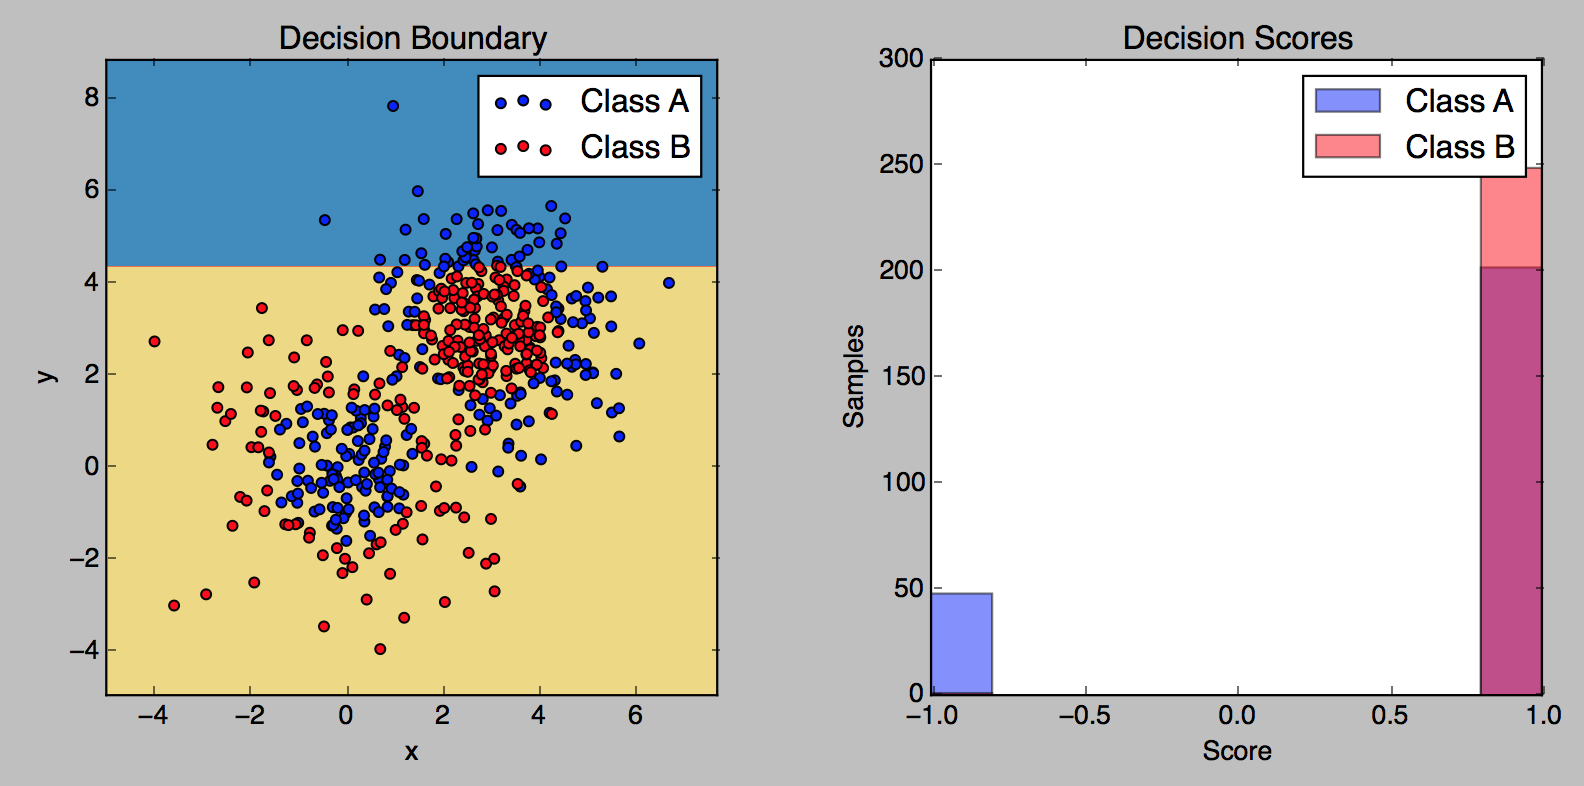
\includegraphics[width=\textwidth]{images/1.png}
		\caption{Abbildung 1: 1 Lerner}
	\end{subfigure}%
	~
	\begin{subfigure}[t]{0.33\textwidth}
		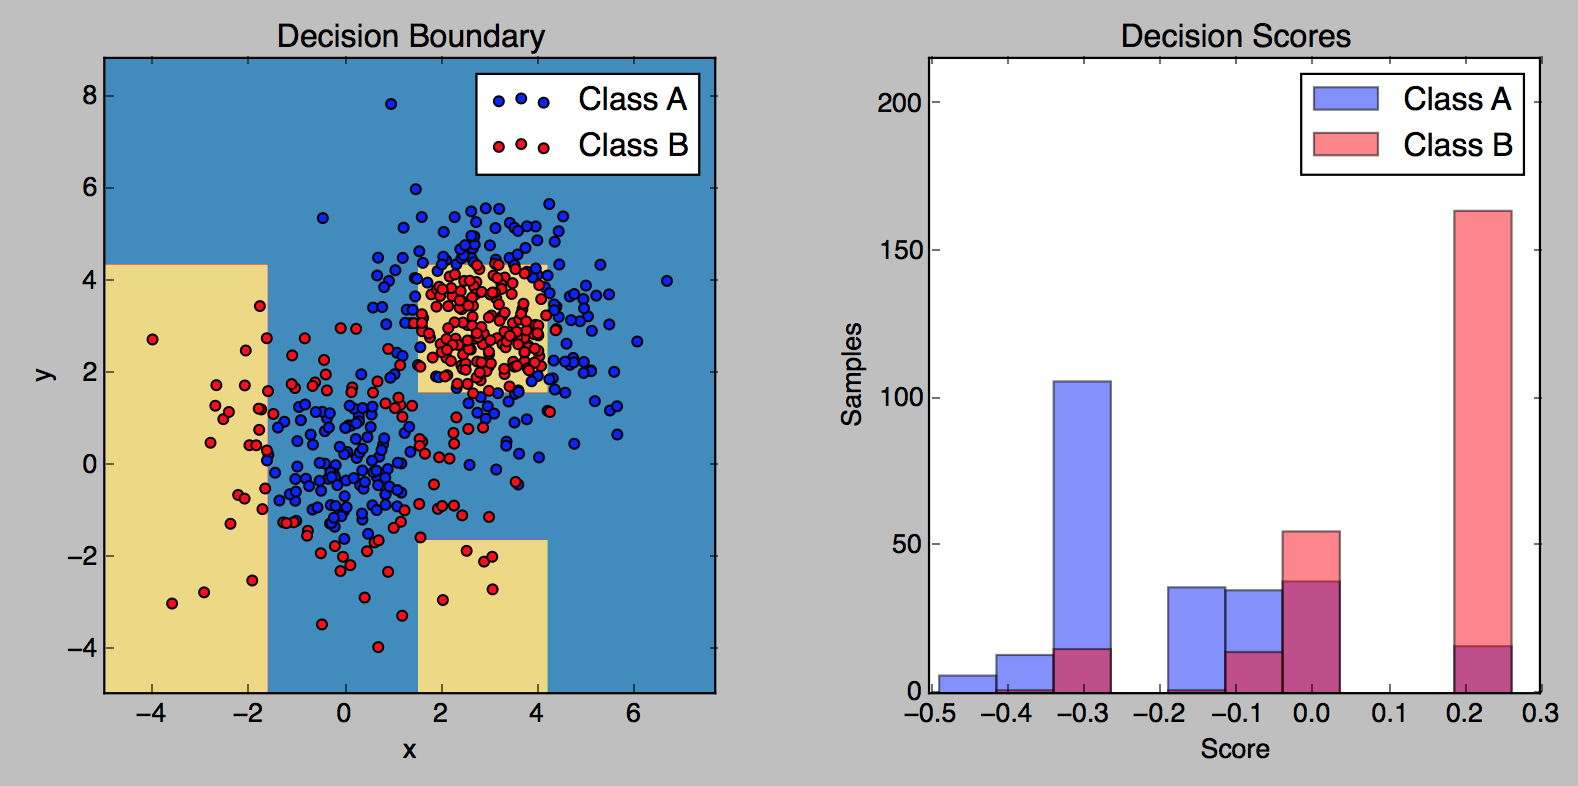
\includegraphics[width=\textwidth]{images/10.png}
		\caption{Abbildung 2: 10 Lerner}
	\end{subfigure}%
	~
	\begin{subfigure}[t]{0.33\textwidth}
		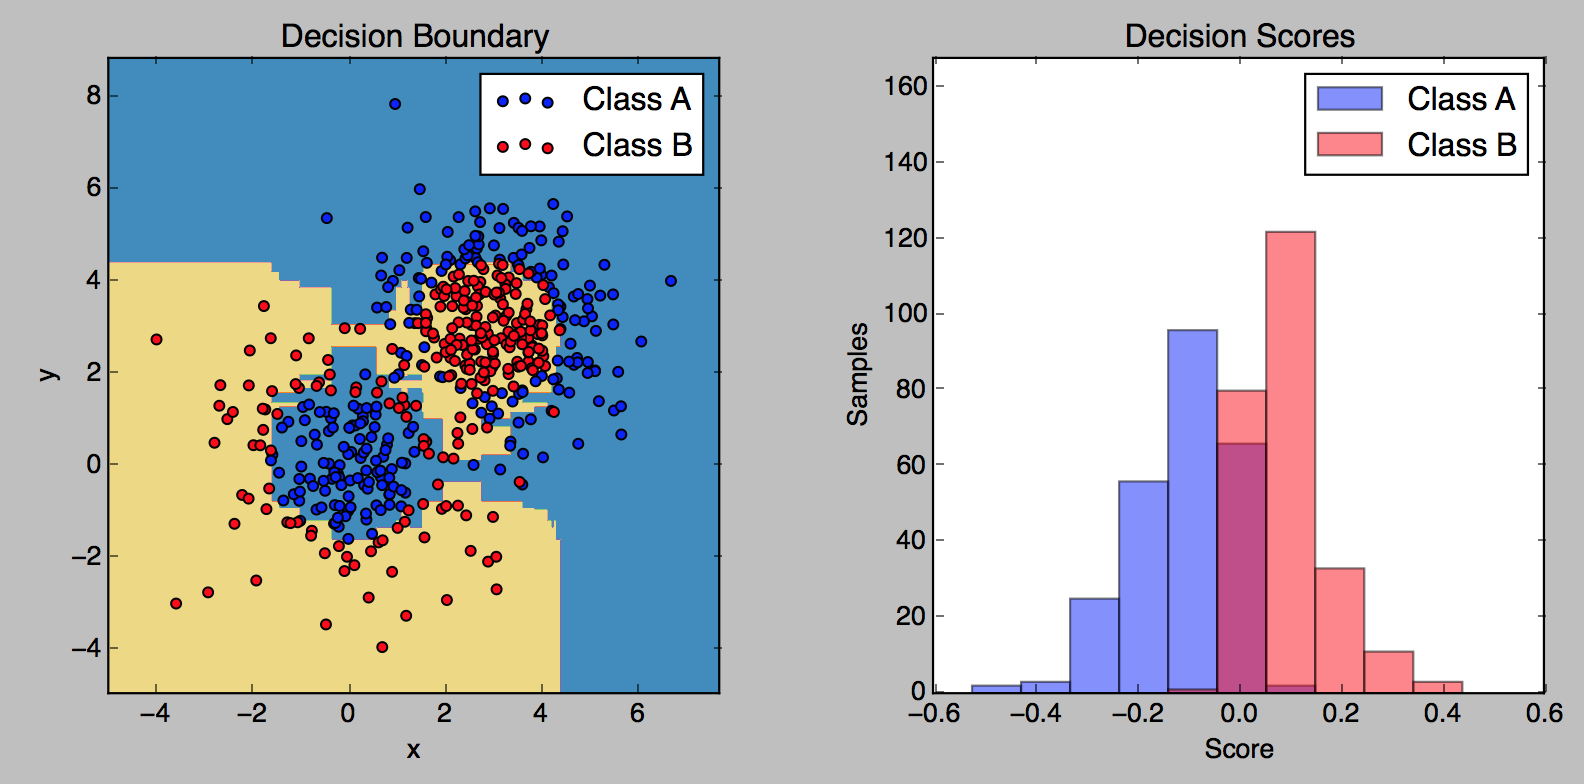
\includegraphics[width=\textwidth]{images/500.png}
		\caption{Abbildung 3: 500 Lerner}
	\end{subfigure}
	
	\caption*{Plots bei verschieden vielen Lernern}
\end{figure*}

AdaBoost nutzt mehrere weak learner (in diesem Beispiel Bäume der Tiefe 1), um zusammen einen strong learner zu bilden. In Abbildung 1 ist zu sehen, dass die Decision Boundary bei einem learner aus einer geraden Linie besteht, welche die Instanzen in 2 Gruppen aufteilt. Im Histogramm ist zu sehen, dass dies zwar dazu führt, dass mehr als die Hälfte der Instanzen richtig klassifiziert werden, aber auch, dass die Fehlerquote sehr hoch ist. Bei 10 Lernern, wie in Abbildung 2 können mehr Instanzen richtig klassifiziert werden, weil der strong learner durch die vielen weak lerner den Merkmalsraum in mehr "`Bereiche"' einteilt, welche im Decision Boundary Diagramm gut zu sehen sind. Diese Bereiche entstehen, weil die hier genutzten weak learner den Merkmalsraum in je 2 Hälften an unterschiedlichen Stellen unterteilen. Im strong learner werden nun, bildlich gesprochen, die weak learner übereinander gelegt. Dabei kommt es zu Überscheidungen von unterschiedlich "`eingefärbten"' Bereichen. Diese bekommen im strong learner jene Klasse zugeteilt, welche in dem betrachteten Bereich mit dem größten Gewicht in den schwachen Lernern vorkommt. Mit ein ausreichend großen Zahl an schwachen Lernern, z.B. 500 wie in Abbildung 3, werden die Decision Boundary komplexer und die Klassifizierung noch genauer. Im Histogramm wird deutlich, dass die "`Sicherheit"' der Aussagen, der Score, mit steigender Anzahl an schwachen Lernern abnimmt, jedoch der strong learner weniger Fehler macht, zum Vergleich, der "`strong learner"' aus einem weak learner klassifizierte etwas über 200 von 500 Instanzen falsch (laut Histogramm aus Abbildung 1), während der strong learner aus Abbildung 3 nur noch etwa 70 Instanzen falsch zuordnet.

\section*{Nr.3}
0.632 Bootstrap meint die Bootstrap-Evaluierung mit einem Testset der Größe n, wobei n die Größe des genutzten Datensatzes ist. Für das Bootstrapverfahren werden zufällig gleichverteilt Instanzen aus dem Datensatz dem Trainingssatz hinzugefügt, bis dieser voll ist. Dabei wird in jeder Iteration der komplette Datensatz betrachtet, inklusive der bereits gewählten Instanzen. Die nicht gewählten Instanzen bilden den Testsatz.
Die Wahrscheinlichkeit, dass eine Instanz in einer Iteration nicht gewählt wird beträgt
\[ 1 - \frac{1}{n}  \]
Die prozentuale Größe des Testsatzes beträgt somit
\[ (1 - \frac{1}{n})^m \]
wobei $n$ die Größe des Datensatzes und $m$ die Größe des Trainingssatzes ist. Für $n = m$ gilt:
\[ 1 - (1 - \frac{1}{n})^n \approx 1 - \frac{1}{e} \approx 0,632 \]
Für einen Testsatz der Größe $2n$  folgt somit:
\[ 1 - (1 - \frac{1}{n})^2n = 1 - \left((1 - \frac{1}{n})^n\right)^2  \approx 1 - \frac{1}{e^2} \approx 0,865 \]

\end{document}